 \chapter{Ponti in AC}
 I \textbf{ponti in alternata} sono strumenti \textbf{analogici} che permettono di calcolare \textbf{impedenze}.
  \begin{center}
    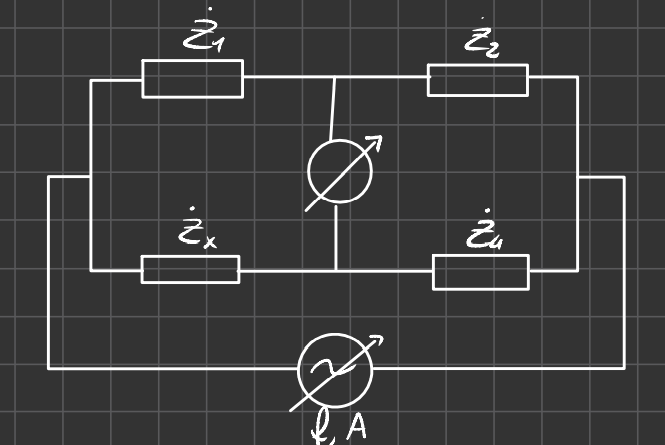
\includegraphics[width=0.50\textwidth]{Images/figure31.png}
  \end{center}
\begin{equation*}
\begin{dcases}
    \dot{Z}_1 \bar{I}_1 =  \dot{Z}_x \bar{I}_x\\
    \dot{Z}_2 \bar{I}_1 =  \dot{Z}_4 \bar{I}_x
\end{dcases}
\implies \dot{Z}_x = \frac{\dot{Z}_1}{\dot{Z}_2} \cdot \dot{Z}_4
\end{equation*}
Quindi ho due equazioni:
\begin{equation*}
\begin{dcases}
    Re\{\dot{Z}_x\} = Re\left(\frac{\dot{Z}_1}{\dot{Z}_2} \cdot \dot{Z}_4\right)\\
    Im\{\dot{Z}_x\} = Im\left(\frac{\dot{Z}_1}{\dot{Z}_2} \cdot \dot{Z}_4\right)
\end{dcases}
\end{equation*}
\begin{equation*}
\begin{dcases}
    |\dot{Z}_x| = \left| \frac{\dot{Z}_1}{\dot{Z}_2} \cdot \dot{Z}_4\right|\\
    \theta_x = \theta_1 + \theta_4 - \theta_2
\end{dcases}
\end{equation*}
Allora possiamo dire che esistono \textbf{due tipologie di ponti}:
\begin{itemize}
    \item \textbf{Prodotto}
    \begin{itemize}
        \item \textbf{Re}
        \item \textbf{Im}
    \end{itemize}
    \item \textbf{Rapporto}
    \begin{itemize}
        \item \textbf{Re}
        \item \textbf{Im}
    \end{itemize}
\end{itemize}
\section{Ponte di Gott (a rapporto reale)}
  \begin{center}
    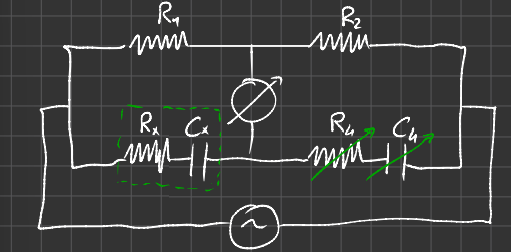
\includegraphics[width=0.50\textwidth]{Images/figure32.png}
  \end{center}
\begin{equation*}
    R_x + \frac{1}{j \w C_x} = \frac{R_1}{R_2} \left(R_4 + \frac{1}{j\w C_4}\right)
\end{equation*}
\begin{equation*}
    \begin{dcases}
        R_x = \frac{R_1}{R_2} \cdot R_4\\
        C_x = \frac{R_2}{R_1} \cdot C_4
    \end{dcases}
    tan(\delta) = \w R_x C_x = \w R_4 C_4
\end{equation*}
\section{Ponte di De Sauty (ponte a rapporto reale)}
  \begin{center}
    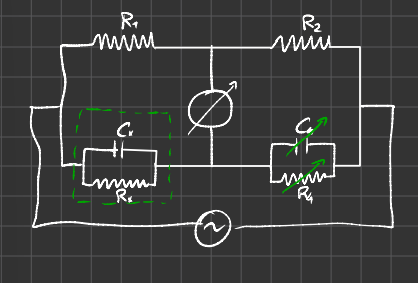
\includegraphics[width=0.50\textwidth]{Images/figure33.png}
  \end{center}
\begin{equation*}
    \dot{Y}_x = \frac{\dot{Z}_2}{\dot{Z}_1}\cdot \dot{Y}_4
\end{equation*}
\begin{equation*}
    \frac{1}{R_x} + j\w C_x = \frac{R_2}{R_1} \left(\frac{1}{R_4} + j \w C_4\right)
\end{equation*}
\begin{equation*}
    \begin{dcases}
        R_x = \frac{R_1}{R_2} R_4\\
        C_x = \frac{R_2}{R_1} C_4
    \end{dcases}
    \implies tan(\delta) = \frac{1}{\w R_x C_x} = \frac{1}{\w R_4 C_4}
\end{equation*}
\section{Ponte di Maxwell (prodotto reale)}
  \begin{center}
    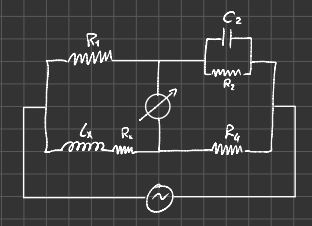
\includegraphics[width=0.50\textwidth]{Images/figure34.png}
  \end{center}
\begin{equation*}
    \underbrace{\theta_1}_{0} + \underbrace{\theta_4}_0 = \underbrace{\theta_2}_{\pm 90} + \underbrace{\theta_x}_{\pm 90}
\end{equation*}
\begin{equation*}
    \begin{dcases}
        R_x = \frac{R_1}{R_2} R_4\\
        L_x = R_1 R_4 C_2
    \end{dcases}
\end{equation*}
  \begin{center}
    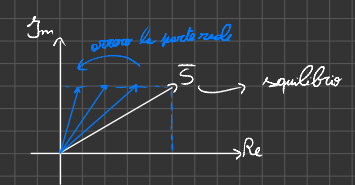
\includegraphics[width=0.50\textwidth]{Images/figure35.png}
  \end{center}
Se vario $R_4$ e $R_2$ tocco sia l'\textbf{equilibrio} di \textbf{parte reale} e sia di \textbf{parte immaginaria}.\\
$\implies$ problema di \textbf{Sliding Balance}
\begin{equation*}
    Q = \frac{\w R_1 R_4 C_4}{\frac{R_1 R_4}{R_2}} = \frac{1}{tan(\delta_2)} = \theta_2
\end{equation*}
\section{Ponte di Schering (prodotto immaginario)}
  \begin{center}
    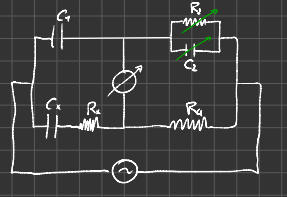
\includegraphics[width=0.50\textwidth]{Images/figure36.png}
  \end{center}
\begin{equation*}
    \underbrace{\theta_x}_{(- 90 , 0)} + \underbrace{\theta_2}_{(- 90 , 0)} = \underbrace{\theta_1}_{- 90} + \underbrace{\theta_4}_{0}
\end{equation*}
\begin{equation*}
    Z_x = \frac{Z_1}{Z_2} Z_4 
\end{equation*}
\begin{equation*}
    R_x + \frac{1}{j \w C_x} = \frac{R_4}{j\w C_1} \left(\frac{1}{R_2} + j \w C_2 \right)
\end{equation*}
\begin{equation*}
    \begin{dcases}
        R_x = \frac{R_4 C_2}{C_1}\\
        C_x = \frac{C_1 R_2}{R_4}
    \end{dcases}
    \implies tan(\delta) = \w R_x C_x = \w R_2 C_2 = \frac{1}{tan(\delta_2)}
\end{equation*}
Che vantaggio c'è? In \textbf{alta frequenza} e in \textbf{alta tensione} un \textbf{condensatore campione} è meglio di \textbf{resistori campioni} (per via di \textbf{parametri parassiti}).\\ \\
Il \textbf{rilevatore di 0} deve anche essere selettivo in caso di alimentazione alternata.
